\chapter{Sample Calculation}
%Had to convert manually
Notebook URL: \url{https://github.com/rdmorgnzation/soilbearing/blob/main/notebooks/sample.ipynb}\\

\begin{python}
#Other imports from library
import resources #Must be 1st line
from blcalc import root_dir
from blcalc.excel_load import BoreholeDataSheets
from blcalc.borehole_parser import BoreholeLog
from blcalc.material import LayerSoil, MaterialData
from blcalc.footing import Footing, FootingType, FootingData
from blcalc.assembly import Assembly
from blcalc.solver import Solver, Methods
from blcalc.geocode import GeoCoder
import pandas as pd
from blcalc.soilproperty import SoilProperty
\end{python}

\begin{python}
filepath = resources.test_data_dir() / "bh1.xls"
\end{python}

\section{Input Files}

\section{Borehole Log}
\url{https://github.com/rdmorgnzation/soilbearing/blob/main/media/media/testdata/bh1.xls}\\

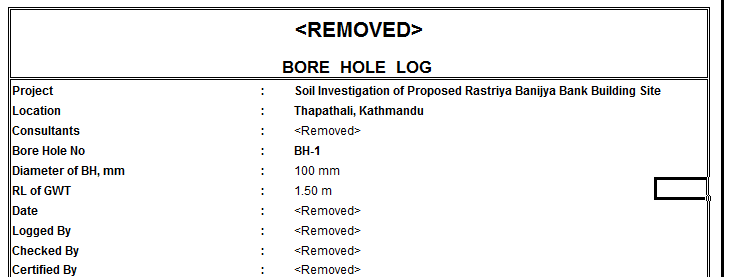
\includegraphics[width=\linewidth,keepaspectratio]{../proj/soilbearing/notebooks/excel_screenshot/1.png}\\\\
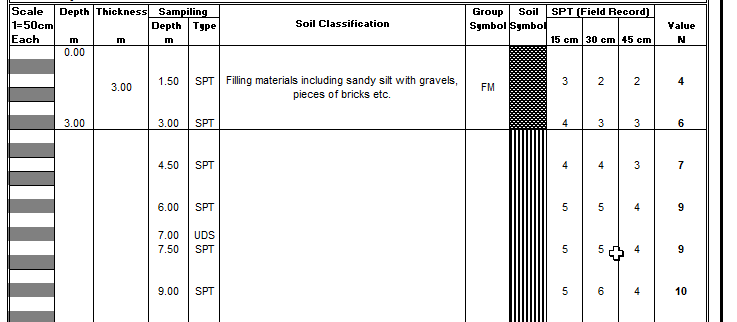
\includegraphics[width=\linewidth,keepaspectratio]{../proj/soilbearing/notebooks/excel_screenshot/2.png}\\\\
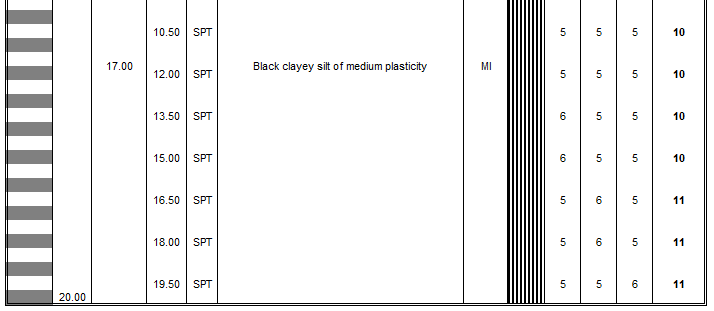
\includegraphics[width=\linewidth,keepaspectratio]{../proj/soilbearing/notebooks/excel_screenshot/3.png}\\\\

\section{Summary Sheet}
\url{https://github.com/rdmorgnzation/soilbearing/blob/main/media/media/testdata/ss.xls}\\

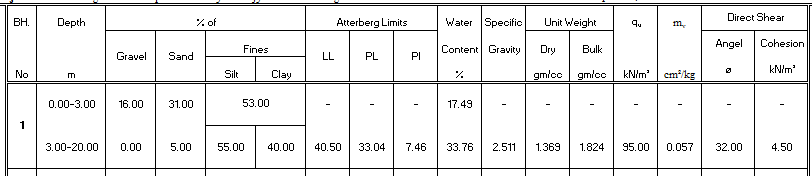
\includegraphics[width=\linewidth,keepaspectratio]{../proj/soilbearing/notebooks/excel_screenshot/ss.png}\\\\

\begin{python}
#Parse it first
sheets = BoreholeDataSheets.load_file(str(filepath.resolve()))
\end{python}

\begin{python}
#Parse 1st sheet
keys = list(sheets.keys())
sheet = sheets[keys[0]]
borehole_log = BoreholeLog(sheet)
\end{python}

\begin{python}
#Attributes obtained from data
pd.DataFrame.from_dict(borehole_log.attributes, orient='index')
\end{python}
Out:\\
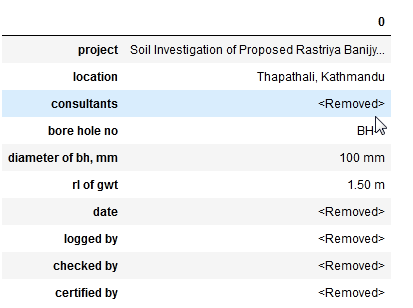
\includegraphics[]{./images/sample/fv.png}\\\\

\begin{python}
#Parsed values
layer=borehole_log.values
#Here i am removing the last value since we used values <20 only,
# For liquefaction. I am trying to get same result as in report
layer = list(filter(lambda x:x[SoilProperty.depth]<20.,layer))
layer = list(filter(lambda x:x[SoilProperty.depth]%1.5==0,layer))
#just for consistancy
pd.DataFrame.from_records(layer)
\end{python}
Out:\\
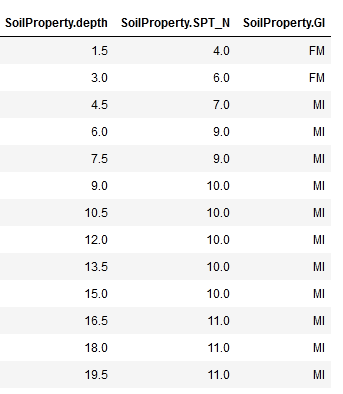
\includegraphics[]{./images/sample/p1.png}\\\\

\begin{python}
geocoder = GeoCoder()
result= geocoder.fetch_geo('Rastriya Banijya Bank, Thapathali, Kathmandu')
#Or use google maps to get result
print('Latitude: ', result[0], '(27.655862)')
print('Longitude: ', result[1], '(85.3064456)')
\end{python}
Out:\\
Latitude:  27.6965195 (27.655862)\\
Longitude:  85.30662 (85.3064456)\\
\\

\section{Add datas from summary sheet}
\begin{python}
#Create footing info based on depth
def get_footing(depth=1.5):
    footing = Footing()
    footing[FootingData.Type] = FootingType.Square
    footing[FootingData.Depth] = depth
    footing[FootingData.Width] = 2
    footing[FootingData.Length] = 2
    return footing
#In our case these values were loaded from excel directly
water_depth = 1.5
for i in layer:
    i[SoilProperty.gamma] = 1.824
    i[SoilProperty.phi] = 32
    i[SoilProperty.qu] = 95
    i[SoilProperty.cu] = 4.5
    i[SoilProperty.G] = 2.511
    if i[SoilProperty.depth]<=3:
        i[SoilProperty.FC] = 53
        i[SoilProperty.water_per] = 0.1749
    else:
        i[SoilProperty.FC] = 95
        i[SoilProperty.water_per] = 0.3376
pd.DataFrame.from_records(layer)
\end{python}
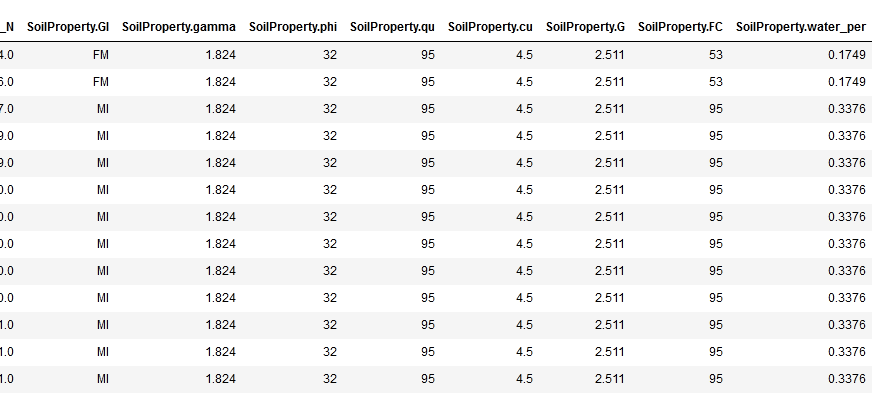
\includegraphics[width=\linewidth,keepaspectratio]{./images/sample/ass.png}\\\\

\section{Values for each layer}
\begin{python}
soil_material = LayerSoil(layer, water_depth, 0)
#Here 0 is for internal purpose (PLAXIS result caching)
pd.DataFrame.from_records(soil_material.get())
\end{python}
Out:\\
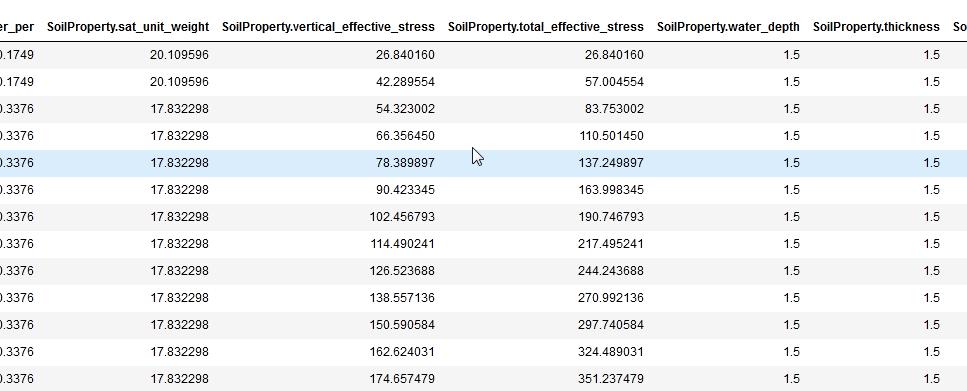
\includegraphics[width=\linewidth,keepaspectratio]{./images/sample/l1.png}\\\\
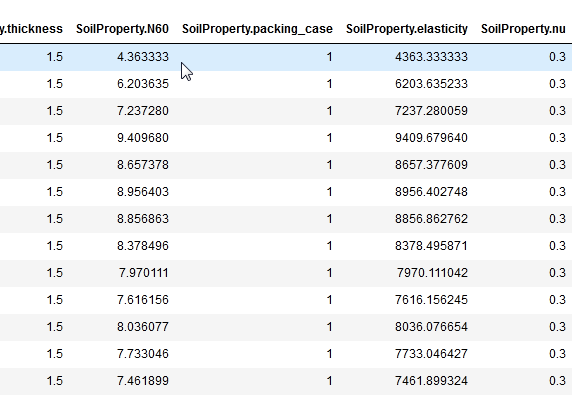
\includegraphics[width=\linewidth,keepaspectratio]{./images/sample/l2.png}\\\\

\textbf{Sample calculation for 1.5m depth}\\

\textbf{Saturated Unit Weight ($\gamma_{sat}$)}\\
= $9.81*\frac{(1+w\%)* G }{ 1+ w\% * G}$
= $9.81*\frac{(1+0.1749)*2.511}{1+0.1749*2.511}$
= 20.10959618\\\\
\textbf{Vertical Effective Stress}=$
\begin{cases}
q + (\gamma_{sat} - 9.81)*depth & ,\text{for below WL}\\
q + \gamma * 9.81 * depth & ,\text{for above WL}
\end{cases}
$\\
So, \textbf{Vertical Effective Stress} = 0 + 1.824 * 9.81 * 1.5 = 26.84016\\

\textbf{Total Effective Stress}=$
\begin{cases}
q + \gamma_{sat} *depth & ,\text{for below WL}\\
q + \gamma * 9.81 * depth & ,\text{for above WL}
\end{cases}
$\\
So, \textbf{Total Effective Stress} = 0 + 1.824 * 9.81 * 1.5 = 26.84016\\

\textbf{Determining N60}

SPT\_N = 4.0

Apply dilatracy correction,\\
Since SPT\_N \textless 15 and above GWT no correction is needed,\\
else, $N = 15 + 0.5 * (SPT\_N - 15)$\\
So, N = 4.0\\
And,\\
Cb = 1\\
Cs = 1\\
Eh = 0.55\\
Cr = 0.7 for depth \textless 3 \\
And, CN = $9.78*\sqrt{\frac{1}{Vertical Effective Stress}} \le 1.7 $\\ = $9.78 * \sqrt{\frac{1}{26.084016}}$ = 1.91492 \textless 1.7 = 1.7\\
So, $N_{60} = Cb*Cs*Eh*Cr*CN*N/0.6 = 1*1*0.55*0.7*1.7*4.0/0.6 = 4.3633333$
\\
\textbf{Packing Case}\\
For sand N60, 4-10, packing case = 2\\
Starting count from 0(computer) = 2-1=1
\\
\textbf{Nu}\\
$\nu$ = 0.3, for cohesionless soil(assumed)
\\
\textbf{Elasticity}\\
$E = 10*N_{60}*100$ = 10 * 4.3633333*100 = 4363.3333\\

\section{Calculation of  BC and LPI}
For 1.5m, avg\_N60 = weighted average N60 from d/2 to 2d
\begin{python}
soil_material.get_avg_N(1.5)
\end{python}
Out:\\
4.363333333333333\\
\begin{python}
footing = get_footing()
assembly = Assembly(footing, soil_material)
solver = Solver(assembly)
results = solver.run()
#print(results)
\end{python}
\subsection{Shear Methods}

\subsubsection{Terzaghi}
$Rw1 = 0.5* (1+water\_depth/depth\_footing) = 1$\\
$Rw2 = 0.5* (1+(water\_depth-depth\_footing)/width\_footing) = 0.5$\\
$q_s = 1.2*c*N_c + surchage*N_q*Rw1 + 0.4*\gamma*9.81*width\_footing*N_\gamma*Rw2$\\
$=1.3*4.5*44.0357+26.840160*28.51657*1+0.4*1.824*9.81*2*28.78*0.5$\\
$=1228.987$\\
$q_{ns} = (q_s - q)/3 = (1228.987-26.84016)/3=400.7157$\\
\begin{python}
results[Methods.Terzaghi]
\end{python}
Out:\\
400.71581138243215

\subsubsection{Meyerhof}
$K_p = tan^2(45+ \phi/2)$ = $tan^2(45+32/2)$ = 3.2546\\
sc = $1 + 0.2*K_p*width\_footing/length\_footing$ = $1+0.2*3.2546*2/2$ = 1.65092\\
$sq=1+0.1*K_p*width\_footing/length\_footing = 1+0.1*3.2546*2/2 = 1.32546$\\
$sy = sq = 1.32546$\\
$dc = 1 +0.2*\sqrt{K_p}*depth\_footing/width\_footing = 1+0.2*\sqrt{3.2546}*1.5/2 = 1.2706$\\
$dq =1 +0.1*\sqrt{K_p}*depth\_footing/width\_footing = 1+0.1*\sqrt{3.2546}*1.5/2 = 1.1353$\\
$dy = dq = 1.1353$\\
$c\_term = cohesion*Nc(phi)*sc*dc = 4.5*35.49026*1.65092*1.2706 = 335.009$\\
$q\_term = surchage*Nq(phi)*sq*dq*Rw1 = 26.84016*23.176776*1.32546*1.1353*1 = 936.0852$\\
$y\_term = 0.5*gamma*9.81*self.width\_footing*Ny(phi)*sy*dy*Rw2 = 0.5*1.824*9.81*2*22.02249*1.32546*1.1353*0.5 = 296.488$\\
$q_s=1567.58248$\\
$q_{ns}=(1567.58248-26.84016)/3=513.58$
\begin{python}
results[Methods.Meyerhof]
\end{python}
Out:\\
513.5822200901385

\subsubsection{Hansen}
$N_c=35.490260$\\
$N_q=23.1767762$\\
$N_y=20.78638$\\
$sc=1+N_q/N_c*width\_footing/length\_footing= 1+23.1767762/35.49026*2/2=1.653046$\\
$sq=1+width\_footing/length\_footing*tan(\phi)=1+2/2*tan(32)=1.624869$\\
$sy=1-0.4*width\_footing/length\_footing=1-0.4*2/2=0.6$\\
$dc = 1 +0.4*width\_footing/length\_footing=1+0.4*2/2=1.4$\\
$dq = 1 +2*tan(\phi)*(1-sin(\phi))^2 * depth\_footing/width\_footing=1+2*tan(32)*(1-sin(32))^2*1.5/2=1.20712$\\
$dy=1$\\
$c\_term = cohesion*N_c*sc*dc=4.5*35.49026*1.653046*1.4=369.6023$\\
$q\_term = surchage*N_q*sq*dq*Rw1=26.84016*23.1767762*1.624869*1.20712*1=1220.1323$\\
$y\_term = 0.5*gamma*9.81*width\_footing*N_y*sy*dy*Rw2=0.5*1.824*9.81*2*20.78638*0.6*1*0.5=111.581953$\\
$q_s = c\_term+q\_term+y\_term=1701.31656$\\
$q_{ns} = (1701.31656 - 26.84016)/3 = 558.158$
\begin{python}
results[Methods.Hansen]
\end{python}
Out:\\
558.1594404871763

\subsubsection{Vesic}
$N_c=35.4902607$\\
$N_q=23.176776$\\
$N_y=30.2146529$\\
$sc=1+N_q/N_c*width\_footing/length\_footing= 1+23.176776/35.4902607*2/2=1.653046$\\
$sq=1+width\_footing/length\_footing*tan(\phi)=1+2/2*tan(32)=1.624869$\\
$sy=1-0.4*width\_footing/length\_footing=1-0.4*2/2=0.6$\\
$dc = 1 +0.4*width\_footing/length\_footing=1+0.4*2/2=1.4$\\
$dq = 1 +2*tan(\phi)*(1-sin(\phi))^2 * depth\_footing/width\_footing=1+2*tan(32)*(1-sin(32))^2*1.5/2=1.20712$\\
$dy=1$\\
$c\_term = cohesion*N_c*sc*dc=4.5*35.49026*1.653046*1.4=369.6023$\\
$q\_term = surchage*N_q*sq*dq*Rw1=26.84016*23.1767762*1.624869*1.20712*1=1220.1323$\\
$y\_term = 0.5*gamma*9.81*width\_footing*N_y*sy*dy*Rw2=0.5*1.824*9.81*2*30.2146529*0.6*1*0.5=162.19322$\\
$q_s = c\_term+q\_term+y\_term=1751.93$\\
$q_{ns} = (1701.31656 - 26.84016)/3 = 575.03$
\begin{python}
results[Methods.Vesic]
\end{python}
Out:\\
575.0298611603204

\subsubsection{Plaxis}
For shear failure in PLAXIS, a large deformation is applied (same result can be obtained by applying large load), so that soil fails by shear. In both cases the soil fails during stagged loading. So we obtain result in plaxis which shows that step failed, but we get result.
\begin{python}
results[Methods.PlaxisShear]
\end{python}
Out:\\
797.05

\subsubsection{Teng}
$q_{ns} = 0.11*N60*N60*width\_footing*Rw2+0.33*(100+N60*N60)*depth\_footing*Rw1$\\
$= 0.11*4.36333^2*2*0.5+0.33*(100+4.36333^2)*1.5*1 = 61.018$
\begin{python}
results[Methods.Teng]
\end{python}
Out:\\
61.01840005555556

\subsection{Settlement Methods}
Take 25mm deflection,

\subsubsection{Meyerhof}
$Rd = 1 + 0.33*depth\_footing/width\_footing = 1+0.33*1.5/2= 1.2475$\\
$b = water\_depth-depth\_footing = 1.5-1.5=0$\\
$Wy = 0.5+0.5*b / width\_footing=0.5$\\
$q_s = 8.1*n60*((width\_footing+0.3)/width\_footing)^2*Wy*Rd$\\
$=8.1*4.3633*((2+0.3)/2)^2*0.5*1.2475=29.154772$
\begin{python}
results[Methods.MeyerhofDeflection]
\end{python}
Out:\\
29.154772040624994

\subsubsection{Bowels}
$q_s = 1.5*Meyerhoff = 1.5*29.154772= 43.732158$
\begin{python}
results[Methods.Bowels]
\end{python}
Out:\\
43.73215806093749

\subsubsection{Peck}
$Cw = 0.5 + 0.5*water\_depth/(depth\_footing+width\_footing) = 0.5+0.5*1.5/(1.5+2) = 0.71429$\\
$q_s =  10.25*Cw*n60 = 10.25*0.71429*4.3633 = 31.94578$
\begin{python}
results[Methods.Peck]
\end{python}
Out:\\
31.945833333333333

\subsubsection{Teng}
$Rd = 1 + depth\_footing/width\_footing = 1 + 1.5/2 = 1.75$\\
$q_s =  35*(n60-3)*((width\_footing+0.3)/(2*width\_footing))^2*Wy*Rd$\\
$ = 35*(4.3633-3)*((2+0.3)/(2*2))^2*0.5*1.75= 13.803945$
\begin{python}
results[Methods.TengDeflection]
\end{python}
Out:\\
13.804282552083333

\subsubsection{Plaxis}
25mm deflection was applied at the footing depth and the corresponding force was taken as bearing capacity.
\begin{python}
results[Methods.Plaxis]
\end{python}
Out:\\
40.06205

\subsection{LPI}
\textbf{Excel sheet}: \url{https://github.com/rdmorgnzation/soilbearing/blob/main/media/media/testdata/lqi.xlsx}
\\
For 1.5m depth,
$FC=94.36$\\
$delN1 = e^(1.63+(9.7/(FC+0.01))-(15.7/(FC+0.01))*(15.7/(FC+0.01)))=5.501985976$\\
$N1cs = N60+delN1 = 20.23473097$\\
$MSF = 0.8758$\\
$Csigma = 1/(18.9-2.55*\sqrt{N1cs}) = 0.134601693$\\
$Ksigma = 1-Csigma*log(vertical\_effective\_stress/100)= 0.921469899$\\
$CRR = exp((N1cs/14.1)+(N1cs/126)^2-(N1cs/23.6)^3+(N1cs/25.4)^3-2.8/1)*(MSF*Ksigma)=0.186699144$\\
$a_g = 0.183$\\
$SRF = exp(-1.012-1.126*sin(depth/11.73+5.133)+8*(0.106+0.118*sin(depth/11.28+5.142)))=0.998325105$\\
$CSR = 0.65*(total\_effective\_stress/vertical\_effective\_stress)*a_g*SRF = 0.118750771$\\
$FS = CRR / CSR = 0.992381257$\\
Since, 0.95<FS<1.2:\\
$Fz = 2e6*exp(-18.427*FS) = 0.022869488$\\
$Wz = 10 - data[SoilProperty.depth]/2 = 9.25$\\
$del\_lpi = Fz * Wz * thickness = 0.317314139$\\
Adding upto depth of 20 we get, LPI = 21.17671875
\begin{python}
results[Methods.Liquifaction]
\end{python}
Out:\\
21.17671874695882
